\documentclass[border=2pt]{standalone}
\usepackage[T1]{fontenc}
\usepackage{libertine}
\usepackage[libertine]{newtxmath}
\usepackage{tikz}
\usetikzlibrary{decorations.pathmorphing,patterns,arrows.meta,calc}
\begin{document}
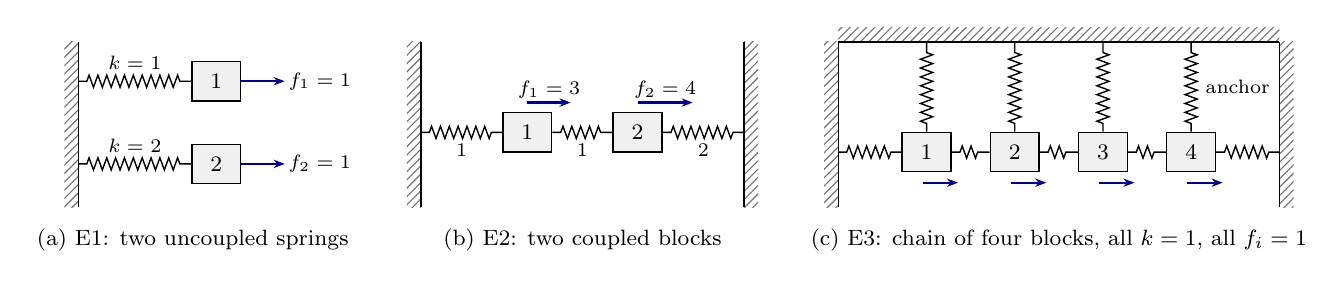
\begin{tikzpicture}[
    x=1cm, y=1cm, font=\footnotesize,
    spring/.style={decorate, decoration={zigzag, segment length=3.2pt, amplitude=2.2pt,
                   pre length=3pt, post length=3pt}, line width=0.5pt},
    block/.style={draw, line width=0.5pt, fill=black!6, minimum width=0.62cm,
                  minimum height=0.5cm, inner sep=0pt},
    force/.style={-{Stealth[length=4pt]}, line width=0.8pt, blue!60!black},
    wall/.style={pattern=north east lines, pattern color=black!55, draw=none},
    lab/.style={font=\scriptsize, inner sep=1pt}]

\begin{scope}
  \fill[wall] (-0.18,-0.35) rectangle (0,1.75);
  \draw[line width=0.6pt] (0,-0.35) -- (0,1.75);
  \node[block] (a1) at (1.75,1.25) {1};
  \draw[spring] (0,1.25) -- (a1.west) node[lab, midway, above=3pt] {$k=1$};
  \draw[force] (a1.east) -- ++(0.55,0) node[lab, right, black] {$f_1=1$};
  \node[block] (a2) at (1.75,0.2) {2};
  \draw[spring] (0,0.2) -- (a2.west) node[lab, midway, above=3pt] {$k=2$};
  \draw[force] (a2.east) -- ++(0.55,0) node[lab, right, black] {$f_2=1$};
  \node[anchor=north, font=\footnotesize] at (1.45,-0.5) {(a) E1: two uncoupled springs};
\end{scope}

\begin{scope}[xshift=4.35cm]
  \fill[wall] (-0.18,-0.35) rectangle (0,1.75);
  \draw[line width=0.6pt] (0,-0.35) -- (0,1.75);
  \fill[wall] (4.1,-0.35) rectangle (4.28,1.75);
  \draw[line width=0.6pt] (4.1,-0.35) -- (4.1,1.75);
  \node[block] (b1) at (1.35,0.6) {1};
  \node[block] (b2) at (2.75,0.6) {2};
  \draw[spring] (0,0.6) -- (b1.west) node[lab, midway, below=3pt] {$1$};
  \draw[spring] (b1.east) -- (b2.west) node[lab, midway, below=3pt] {$1$};
  \draw[spring] (b2.east) -- (4.1,0.6) node[lab, midway, below=3pt] {$2$};
  \draw[force] ($(b1.north)+(0,0.12)$) -- ++(0.55,0) node[lab, above, midway, black] {$f_1=3$};
  \draw[force] ($(b2.north)+(0,0.12)$) -- ++(0.7,0) node[lab, above, midway, black] {$f_2=4$};
  \node[anchor=north, font=\footnotesize] at (2.05,-0.5) {(b) E2: two coupled blocks};
\end{scope}

\begin{scope}[xshift=9.65cm]
  \fill[wall] (-0.18,-0.35) rectangle (0,1.75);
  \draw[line width=0.6pt] (0,-0.35) -- (0,1.75);
  \fill[wall] (5.6,-0.35) rectangle (5.78,1.75);
  \draw[line width=0.6pt] (5.6,-0.35) -- (5.6,1.75);
  \fill[wall] (0,1.75) rectangle (5.6,1.93);
  \draw[line width=0.6pt] (0,1.75) -- (5.6,1.75);
  \foreach \i/\x in {1/1.12, 2/2.24, 3/3.36, 4/4.48} {
    \node[block] (c\i) at (\x,0.35) {\i};
    \draw[spring] (c\i.north) -- (\x,1.75);
    \draw[force] ($(c\i.south)+(-0.05,-0.13)$) -- ++(0.45,0);
  }
  \draw[spring] (0,0.35) -- (c1.west);
  \draw[spring] (c1.east) -- (c2.west);
  \draw[spring] (c2.east) -- (c3.west);
  \draw[spring] (c3.east) -- (c4.west);
  \draw[spring] (c4.east) -- (5.6,0.35);
  \node[lab, anchor=west] at (4.62,1.18) {anchor};
  \node[anchor=north, font=\footnotesize] at (2.8,-0.5) {(c) E3: chain of four blocks, all $k=1$, all $f_i=1$};
\end{scope}
\end{tikzpicture}
\end{document}
